\documentclass[12pt,a4paper]{article}

\usepackage{graphicx}  
\usepackage[margin=2.5cm]{geometry}
\usepackage{breakcites}
\usepackage{indentfirst}
\usepackage{pgfgantt}
\usepackage{pdflscape}
\usepackage{float}
\usepackage{epsfig}
\usepackage{epstopdf}
\usepackage[cmex10]{amsmath}
\usepackage{stfloats}
\usepackage{multirow}
\usepackage{mathtools}

\renewcommand{\refname}{REFERENCES}
\linespread{1.3}

\thispagestyle{empty}


\usepackage{listings}
\usepackage{xcolor}

% Verilog için özel renk ayarları
\lstset{
    language=Verilog,
    basicstyle=\small\ttfamily,
    keywordstyle=\color{blue}\bfseries,
    commentstyle=\color{green!60!black},
    stringstyle=\color{purple},
    numbers=left,
    numberstyle=\tiny,
    stepnumber=1,
    frame=single,
    breaklines=true,
    captionpos=b % Başlığı alta koyar
}

\begin{document}
\nocite{*}
\begin{titlepage}
\begin{center}

\textbf{}\\
\textbf{\Large{ISTANBUL TECHNICAL UNIVERSITY}}\\
\vspace{0.5cm}
\textbf{\Large{COMPUTER ENGINEERING DEPARTMENT}}\\
\vspace{2cm}
\textbf{\Large{BLG 242E\\ DIGITAL CIRCUITS LABORATORY\\ EXPERIMENT REPORT}}\\
\vspace{2.8cm}
\begin{table}[ht]
\centering
\Large{
\begin{tabular}{lcl}
\textbf{EXPERIMENT NO}  & : & 2 \\
\textbf{EXPERIMENT DATE}  & : & 02.03.2026 \\
\textbf{LAB SESSION}  & : & MONDAY - 13.30 \\
\textbf{GROUP NO}  & : & G3 \\
\end{tabular}}
\end{table}
\vspace{1cm}
\textbf{\Large{GROUP MEMBERS:}}\\
\begin{table}[ht]
\centering
\Large{
\begin{tabular}{rcl}
150230089  & : & HÜSEYİN \ TEKE \\
150230033  & : & KUTAY YEKTA \ GENÇOĞLU \\
15021044  & : & HASAN BARIŞ \ ÇALIŞKAN \\

\end{tabular}}
\end{table}
\vspace{2.8cm}
\textbf{\Large{SPRING 2026}}

\end{center}

\end{titlepage}

\thispagestyle{empty}
\addtocontents{toc}{\contentsline {section}{\numberline {}FRONT COVER}{}}
\addtocontents{toc}{\contentsline {section}{\numberline {}CONTENTS}{}}
\setcounter{tocdepth}{4}
\tableofcontents
\clearpage

\setcounter{page}{1}

\section{INTRODUCTION}
The objective of this experiment is to design and implement complex combinational logic circuits using Verilog HDL on the Basys 3 FPGA board. The design process focuses on using combinational \texttt{always@(*)} blocks to realize various digital modules such as multiplexers, decoders, and encoders. Key concepts include the application of Verilog operators, understanding the hardware configuration of common anode seven-segment displays, and managing FPGA pin constraints.

\section{MATERIALS AND METHODS}
All designs were implemented in Verilog and targeted for the Artix-7 FPGAs.

\subsection{8:1 Multiplexer}
An 8:1 multiplexer was designed to route one of eight input lines (\texttt{in[7:0]}) to a single output \texttt{y} based on 3-bit select lines (\texttt{sel[2:0]}). As per the experiment requirements, the circuit was implemented using nested \texttt{if-else} structures within an \texttt{always@(*)} block instead of \texttt{switch-case} statements.
\begin{lstlisting}[caption={8:1 Mux Verilog Implementation}, label={code:Mux}]
always @(*) begin
    if      (FunSel == 3'b000) LED = sw[0];
    else if (FunSel == 3'b001) LED = sw[1];
    else if (FunSel == 3'b010) LED = sw[2];
    else if (FunSel == 3'b011) LED = sw[3];
    else if (FunSel == 3'b100) LED = sw[4];
    else if (FunSel == 3'b101) LED = sw[5];
    else if (FunSel == 3'b110) LED = sw[6];
    else                   LED = sw[7]; 
end
\end{lstlisting}
\subsection{BCD to 7-Segment Decoder}
A 4-bit BCD-to-7-segment decoder was developed to drive the segments \texttt{a-g} of the Basys 3 display. The mapping for digits 0-9 was defined using \texttt{case} statements. The design specifically accounts for the common anode configuration, where segments are active-low. For invalid BCD values (greater than 9), all segments were driven to a specific invalid pattern.
\begin{lstlisting}[caption={BCD to 7 Segment Display implementation}, label={code:BCD to 7 Segment}]
module BCDto7Segment(
    input wire [3:0] sw,
    output reg [6:0] seg,
    output reg dp,
    output reg an
    );
    /**
      an = anode
      reg[0] = A
      reg[1] = B
      reg[2] = C
      reg[3] = D
      reg[4] = E
      reg[5] = F
      reg[6] = G
      dp = DP
    **/
    always@(*)
    begin
        case(sw)
        4'b0000 : 
        begin an = 1; dp = 1; seg = 7'b1000000;
        end
        4'b0001 : 
        begin an = 1; dp = 1; seg = 7'b1111001;
        end 
        4'b0010 : 
        begin an = 1; dp = 1; seg = 7'b0100100;
        end 
        4'b0011 : 
        begin an = 1; dp = 1; seg = 7'b0110000;
        end
        4'b0100 : 
        begin an = 1; dp = 1; seg = 7'b0011001;
        end
        4'b0101 : 
        begin an = 1;  dp = 1; seg = 7'b0110000;
        end
        4'b0110 : 
        begin an = 1; dp = 1; seg = 7'b000010;
        end
        4'b0111 :
        begin an = 1; dp = 1; seg = 7'b1111000;
        end
        4'b1000 : 
        begin an = 1; dp = 1; seg = 7'b0000000;
        end
        4'b1001 : 
        begin an = 1; dp = 1; seg = 7'b0010000;
        end
        default :
        begin an = 1; dp = 1; seg = 7'b1111111;
        end
        endcase
    end
endmodule
\end{lstlisting}
\vfill
\subsection{3:8 Decoder}
A 3:8 decoder was implemented with a 3-bit input (\texttt{in[2:0]}) and 8-bit output (\texttt{out[7:0]}). The logic ensures that only one output line is active (high) for a given input value. The module was constructed using a single \texttt{always@(*)} block with \texttt{if-else} conditions to match each possible input value from 0 to 7.
\begin{lstlisting}[caption={3:8 Decoder Verilog Implementation}, label={code:decoder}]
module decoder_3to8(
    input [2:0] in,
    output reg [7:0] out
);
    always @(*) begin
        if (in == 3'b000) out = 8'b00000001;
        else if (in == 3'b001) out = 8'b00000010;
        else if (in == 3'b010) out = 8'b00000100;
        else if (in == 3'b011) out = 8'b00001000;
        else if (in == 3'b100) out = 8'b00010000;
        else if (in == 3'b101) out = 8'b00100000;
        else if (in == 3'b110) out = 8'b01000000;
        else if (in == 3'b111) out = 8'b10000000;
        else out = 8'b00000000;
    end
endmodule
\end{lstlisting}
\vfill

\subsection{Elaborated Design of all modules}
The schematic generated by the Vivado Synthesis tool provides a visual representation of the logic gates and routing implemented by the Verilog code.

\begin{figure}[H]
    \centering
    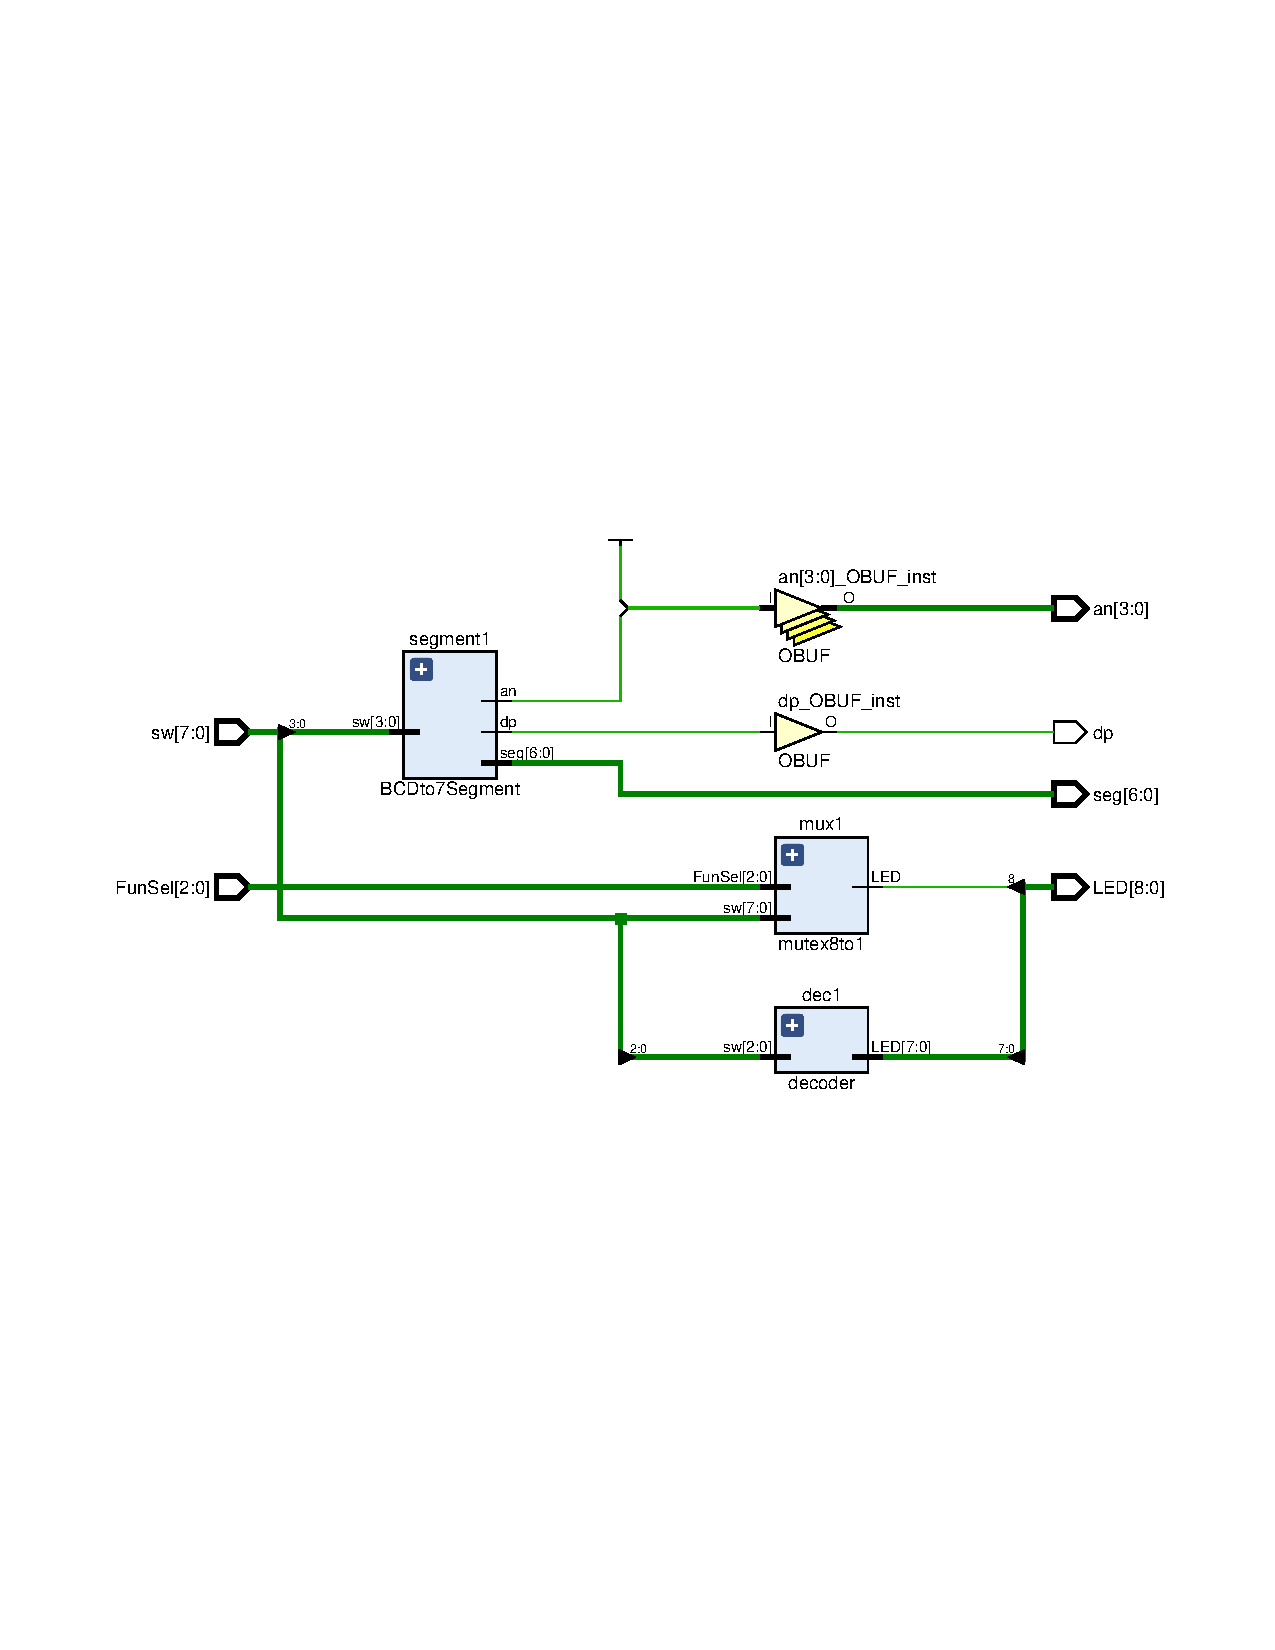
\includegraphics[width=0.9\textwidth]{schematic.pdf}
    \caption{Elaborated Design schematic of the all modules.}
    \label{fig:elaborated}
\end{figure}


\section{RESULTS}
The designs were verified through functional simulations and hardware testing.
\begin{itemize}
    \item \textbf{Simulation:} Waveforms were generated to confirm correct output for all valid input ranges.
    \begin{figure}[H] % [H] resmi tam bu noktaya sabitler
    \centering    % Resmi yatayda ortalar
    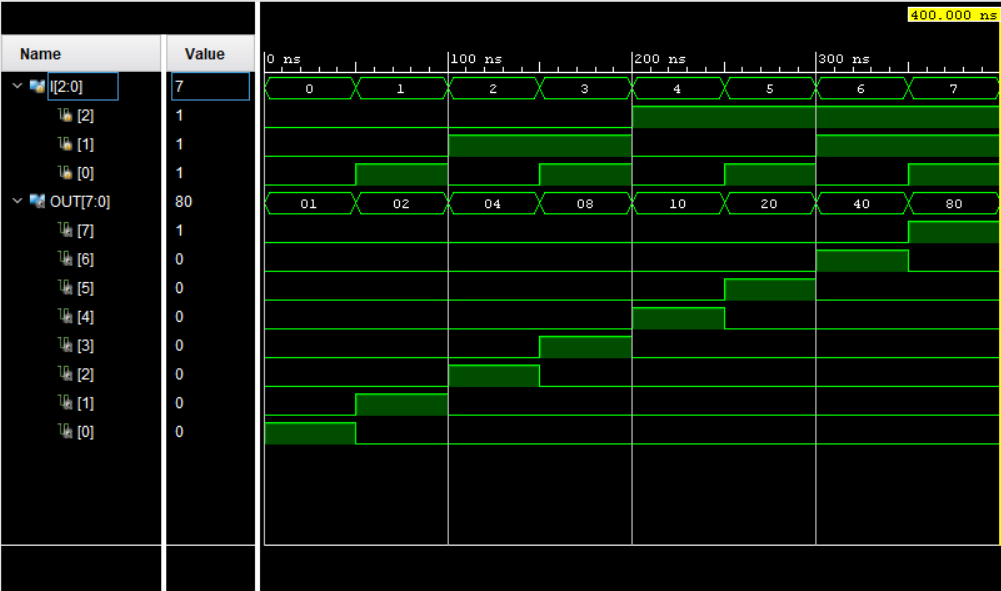
\includegraphics[width=0.8\textwidth]{decoder.png} 
    % width: Resmin genişliğini ayarlar (0.8\textwidth sayfa genişliğinin %80'i demektir)
    % resim_adi.png: Overleaf'e yüklediğiniz dosyanın tam adı
    
    \caption{Decoder Simulation Results} % Resim altı açıklaması
    \label{fig:resim_etiketi} % Metin içinde gönderme yapmak için (örn: Şekil \ref{fig:resim_etiketi})
\end{figure}

    \begin{figure}[H] % [H] resmi tam bu noktaya sabitler
    \centering    % Resmi yatayda ortalar
    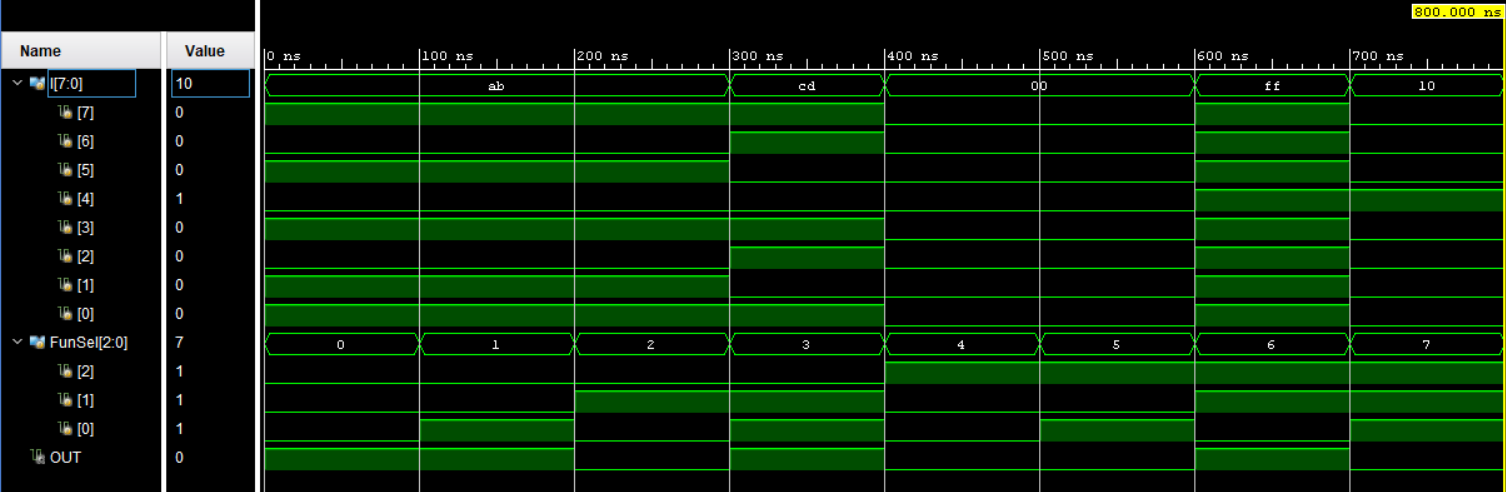
\includegraphics[width=0.8\textwidth]{mux.png} 
    % width: Resmin genişliğini ayarlar (0.8\textwidth sayfa genişliğinin %80'i demektir)
    % resim_adi.png: Overleaf'e yüklediğiniz dosyanın tam adı
    
    \caption{8:1 Multiplexer Simulation Results} % Resim altı açıklaması
    \label{fig:resim_etiketi} % Metin içinde gönderme yapmak için (örn: Şekil \ref{fig:resim_etiketi})
\end{figure}



    \begin{figure}[H] % [H] resmi tam bu noktaya sabitler
    \centering    % Resmi yatayda ortalar
    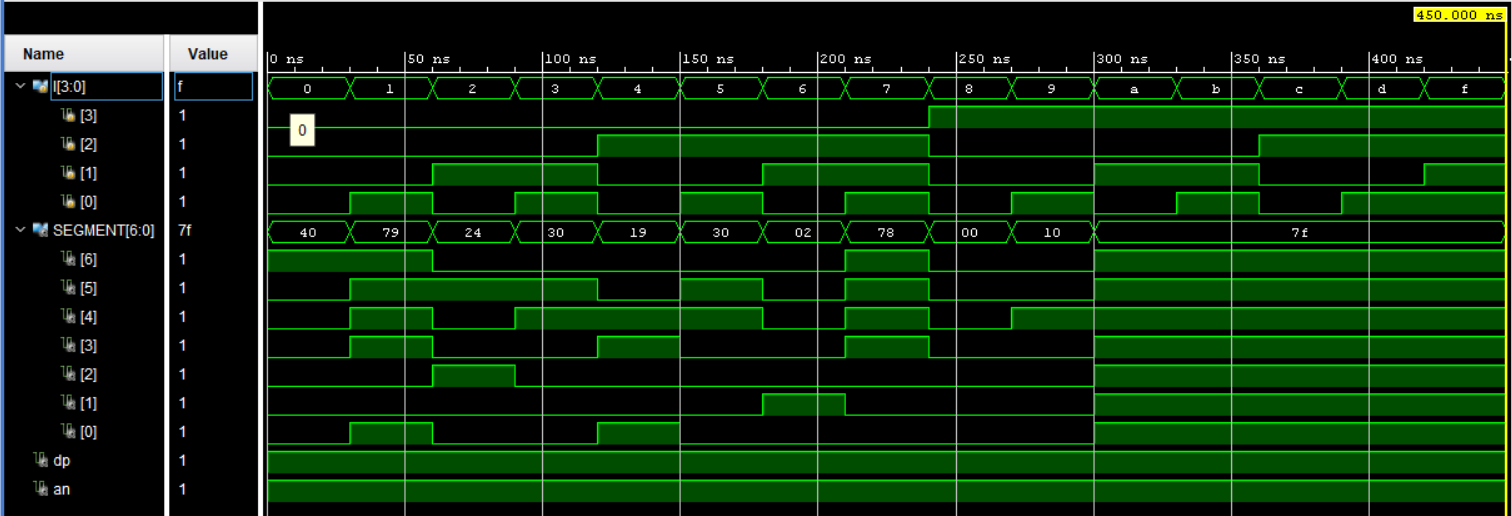
\includegraphics[width=0.8\textwidth]{bcd.png} 
    % width: Resmin genişliğini ayarlar (0.8\textwidth sayfa genişliğinin %80'i demektir)
    % resim_adi.png: Overleaf'e yüklediğiniz dosyanın tam adı
    
    \caption{BCD Segment Simulation Results} % Resim altı açıklaması
    \label{fig:resim_etiketi} % Metin içinde gönderme yapmak için (örn: Şekil \ref{fig:resim_etiketi})
\end{figure}
    \item \textbf{Synthesis:} The synthesis reports indicate the resource usage, including the number of Look-Up Tables (LUTs) and carry logic utilized on the FPGA.
    \item \textbf{Hardware:} The inputs were mapped to DIP switches and outputs to the 7-segment display and LEDs to confirm real-time functionality.

    \begin{figure}[H] % [H] resmi tam bu noktaya sabitler
    \centering    % Resmi yatayda ortalar
    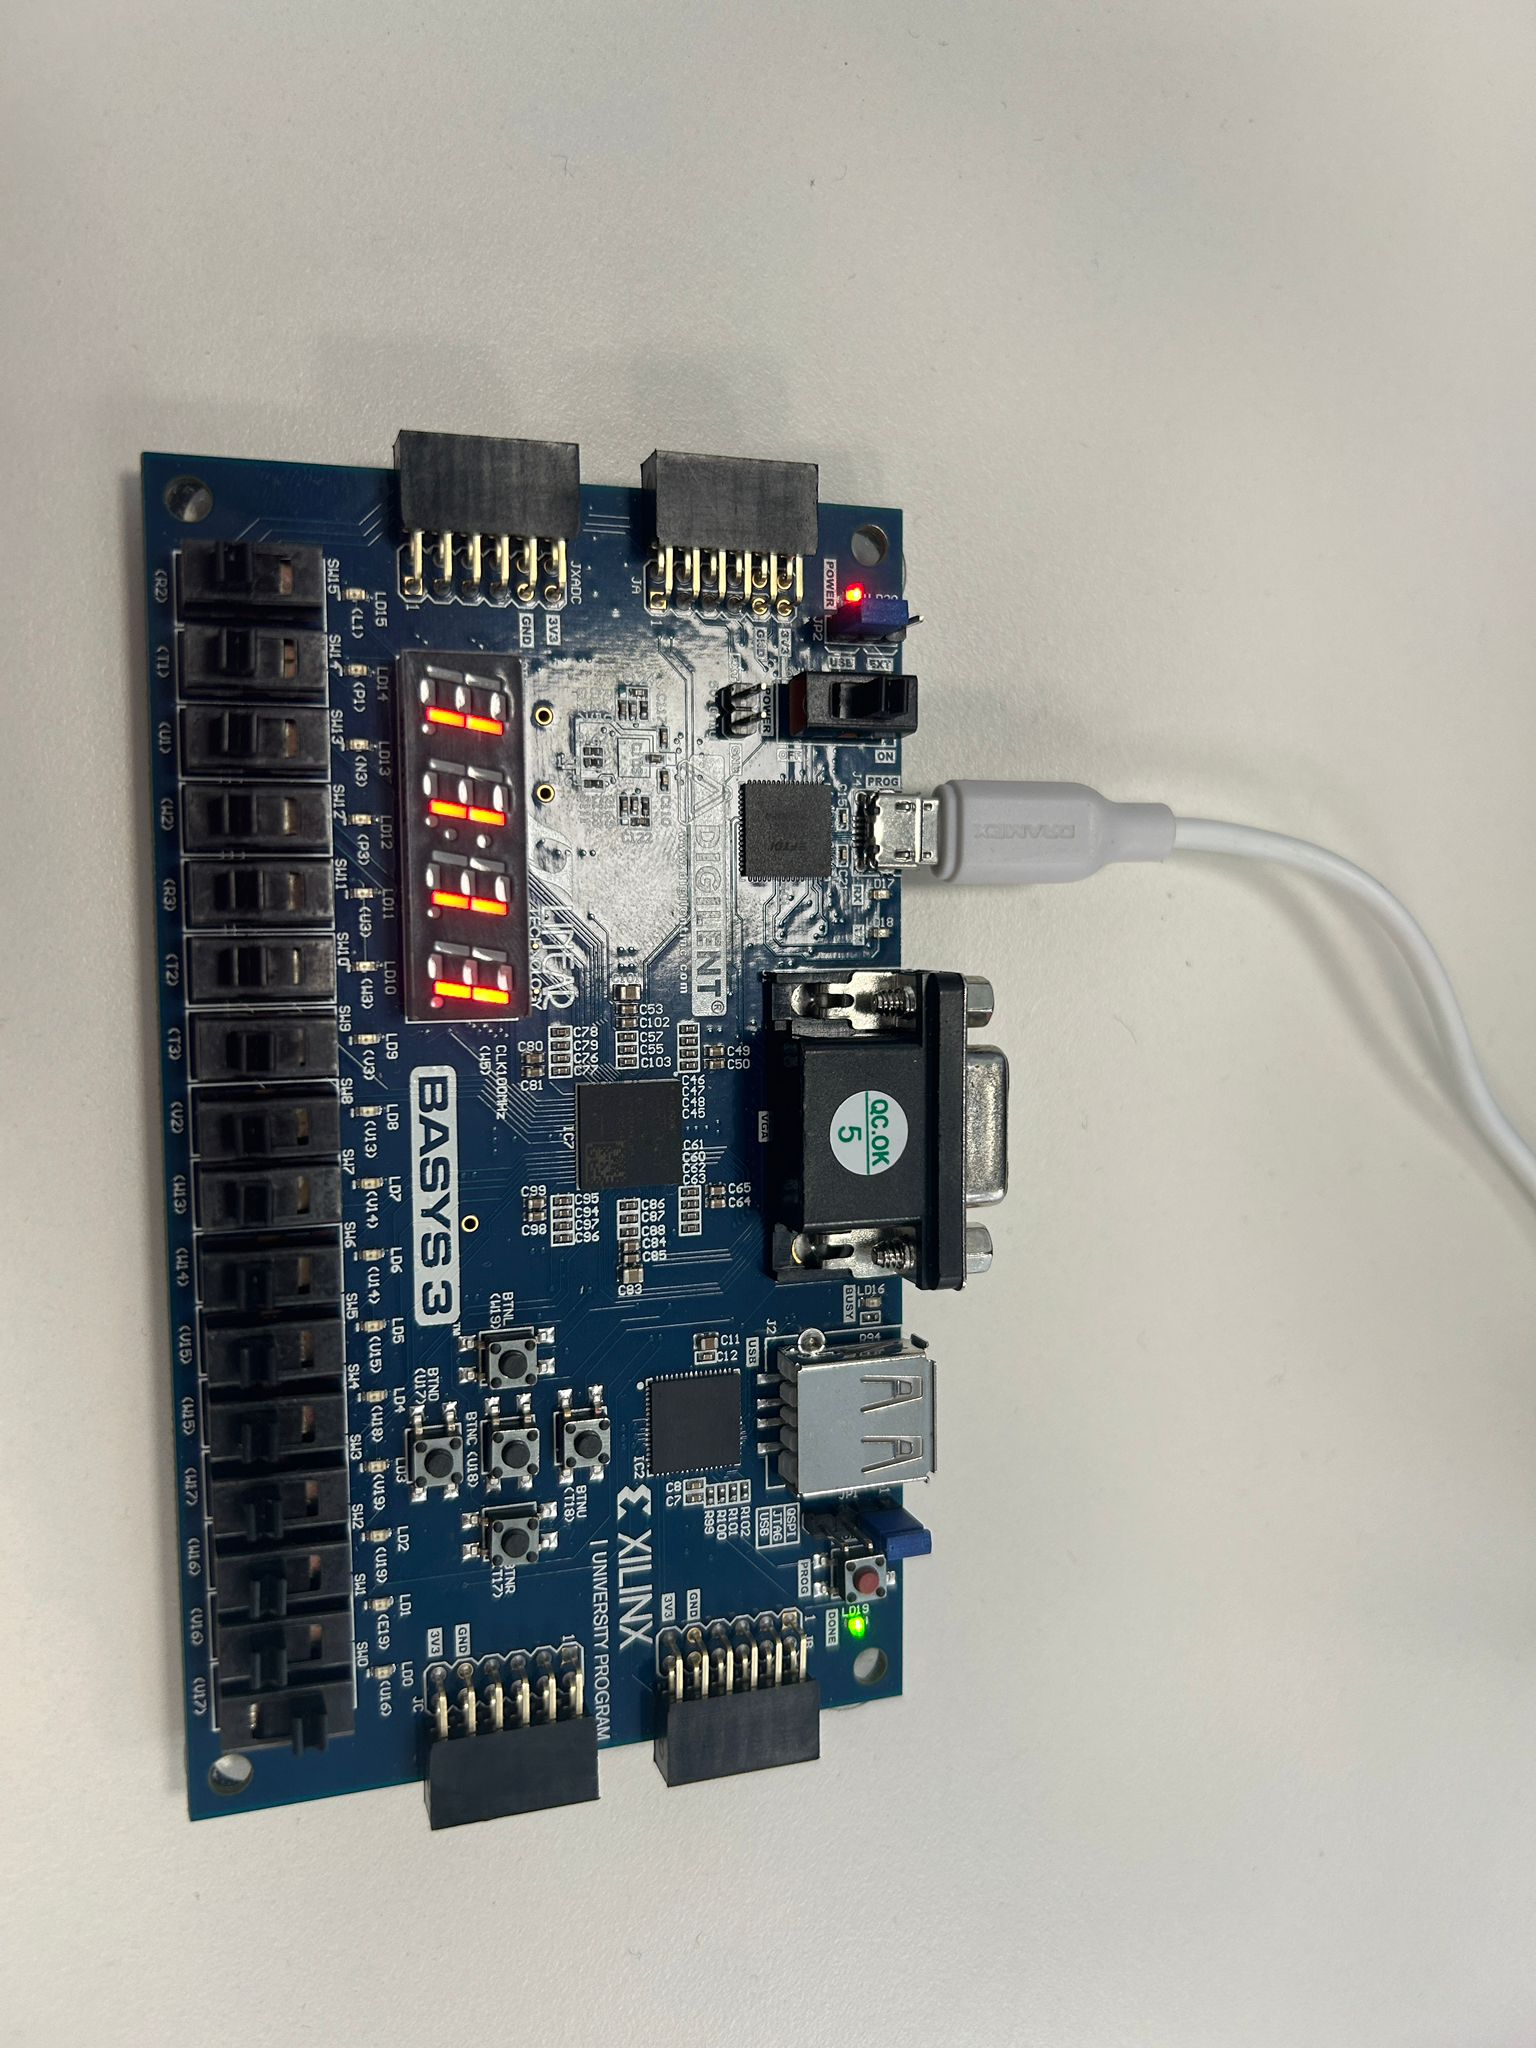
\includegraphics[width=0.8\textwidth]{one.jpeg} 
    % width: Resmin genişliğini ayarlar (0.8\textwidth sayfa genişliğinin %80'i demektir)
    % resim_adi.png: Overleaf'e yüklediğiniz dosyanın tam adı
    
    \caption{BCD Segment hardware result (one)} % Resim altı açıklaması
    \label{fig:resim_etiketi} % Metin içinde gönderme yapmak için (örn: Şekil \ref{fig:resim_etiketi})
\end{figure}


    \begin{figure}[H] % [H] resmi tam bu noktaya sabitler
    \centering    % Resmi yatayda ortalar
    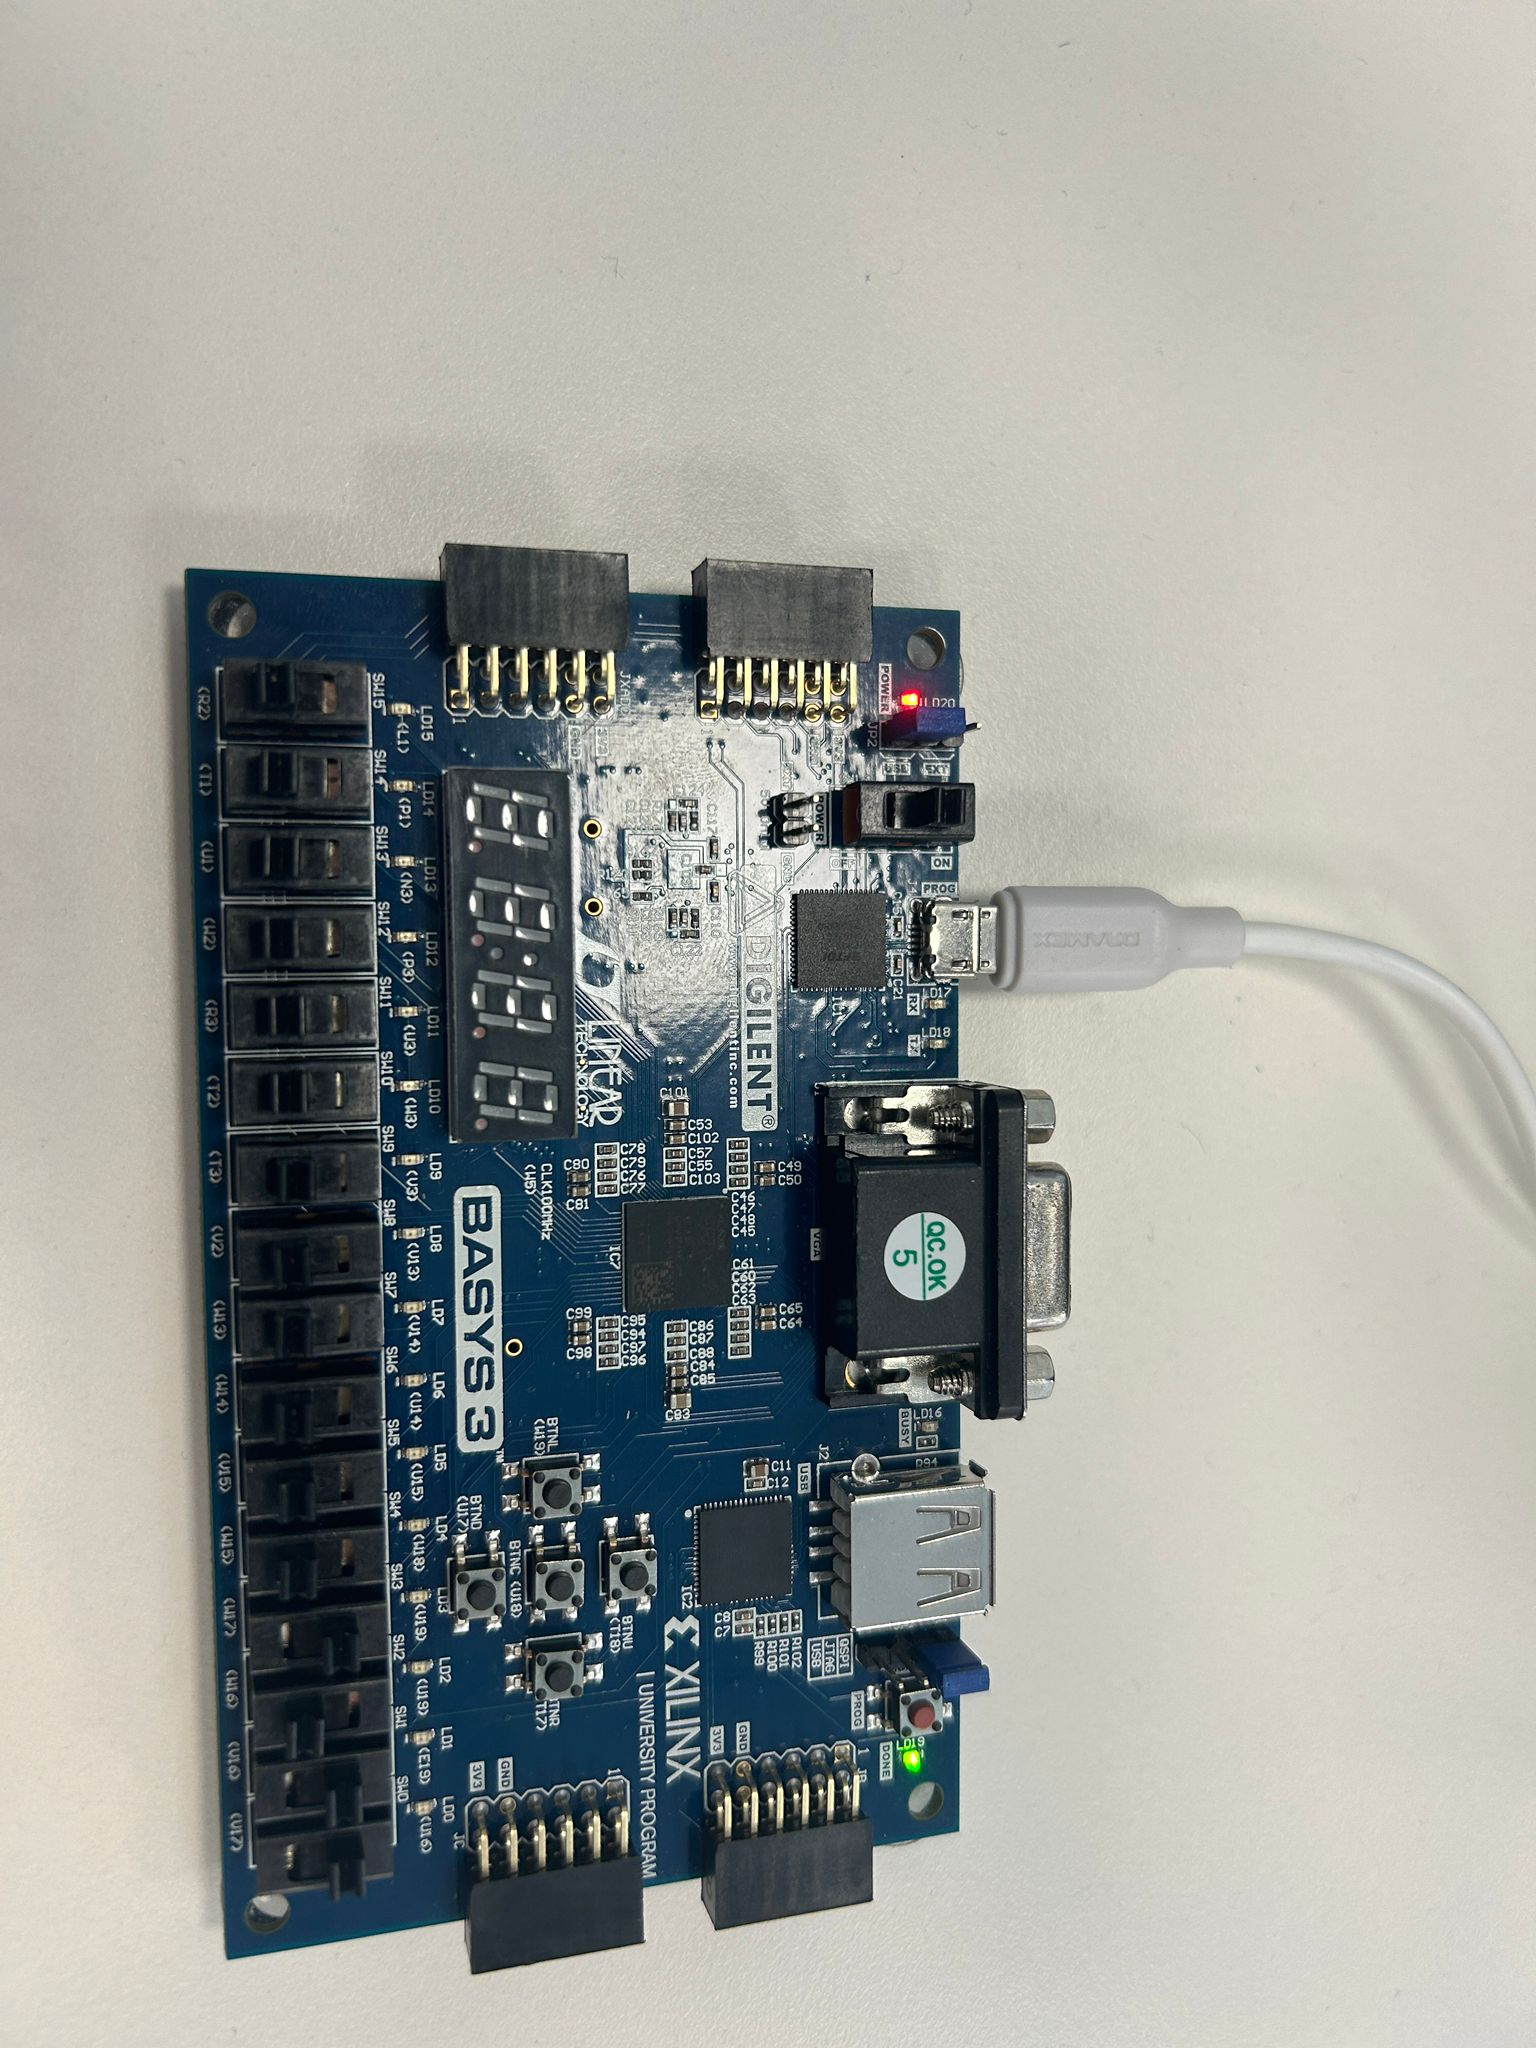
\includegraphics[width=0.8\textwidth]{empty.jpeg} 
    % width: Resmin genişliğini ayarlar (0.8\textwidth sayfa genişliğinin %80'i demektir)
    % resim_adi.png: Overleaf'e yüklediğiniz dosyanın tam adı
    
    \caption{BCD Segment hardware result (undefined input)} % Resim altı açıklaması
    \label{fig:resim_etiketi} % Metin içinde gönderme yapmak için (örn: Şekil \ref{fig:resim_etiketi})
\end{figure}



    \begin{figure}[H] % [H] resmi tam bu noktaya sabitler
    \centering    % Resmi yatayda ortalar
    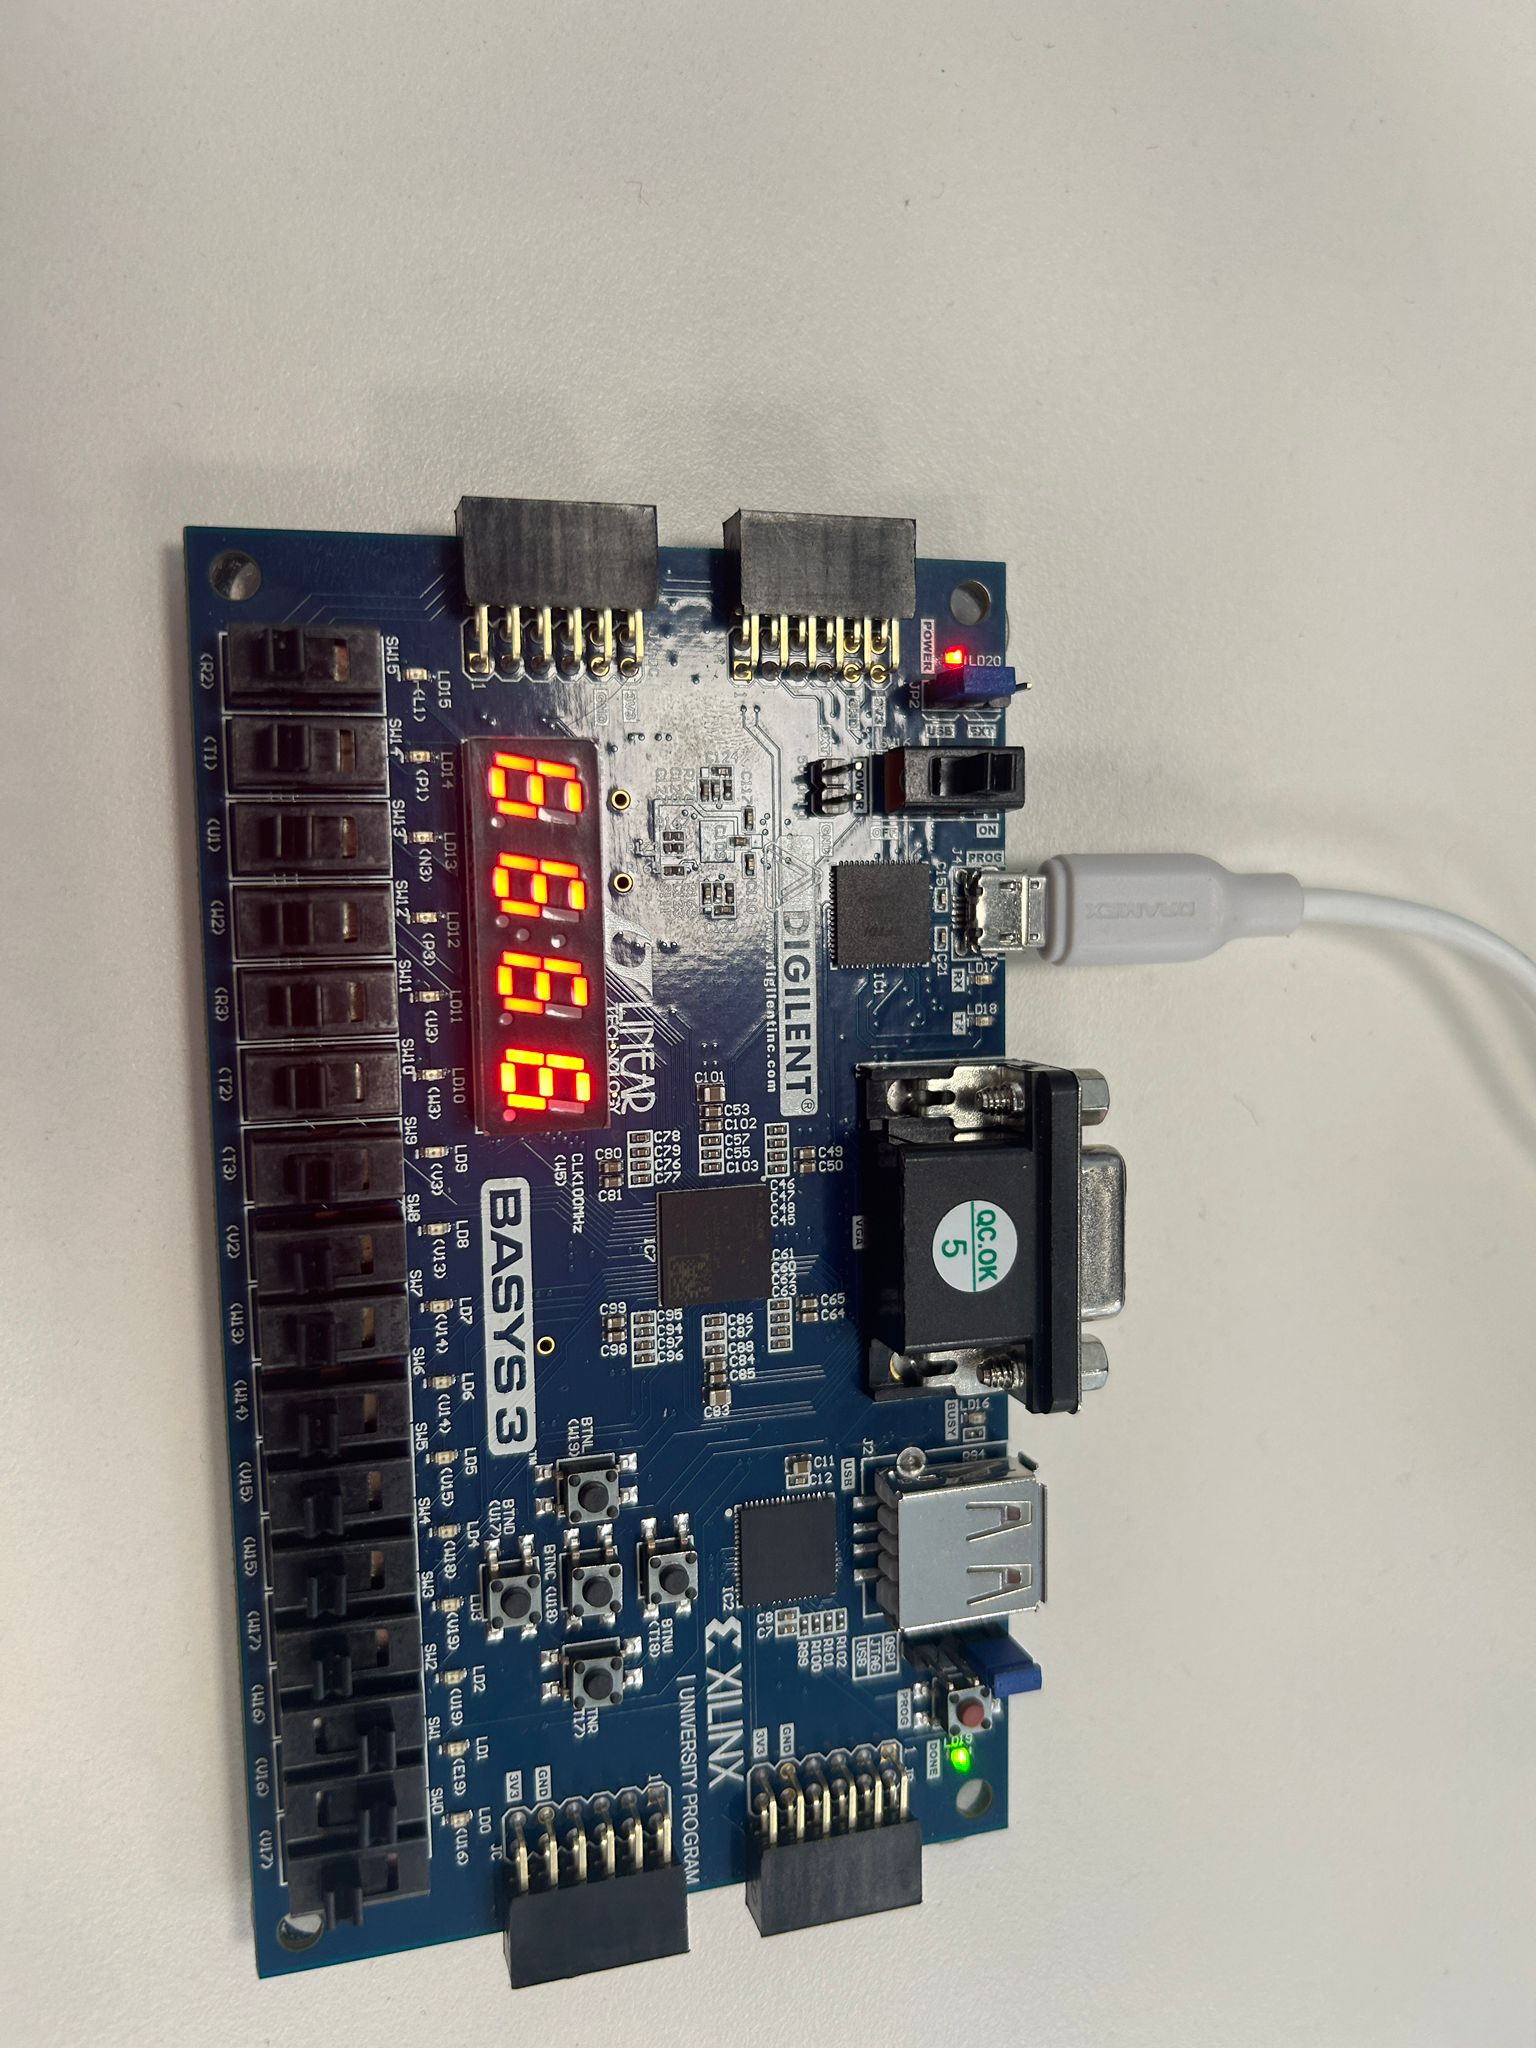
\includegraphics[width=0.8\textwidth]{six.jpeg} 
    % width: Resmin genişliğini ayarlar (0.8\textwidth sayfa genişliğinin %80'i demektir)
    % resim_adi.png: Overleaf'e yüklediğiniz dosyanın tam adı
    
    \caption{BCD Segment hardware result (six)} % Resim altı açıklaması
    \label{fig:resim_etiketi} % Metin içinde gönderme yapmak için (örn: Şekil \ref{fig:resim_etiketi})
\end{figure}
    
\end{itemize}

\section{DISCUSSION}
The implementation demonstrated the priority logic inherent in nested \texttt{if-else} structures, which was particularly evident in the multiplexer design. A critical observation was the active-low requirement for the seven-segment display segments due to the common anode hardware configuration. Properly mapping the internal HDL signals to the physical FPGA pins using the constraints file was essential for correct hardware operation.

\section{CONCLUSION}
In this experiment, complex combinational circuits were successfully synthesized and tested on the Basys 3 board. Through the design of the BCD decoder and adder-subtractor, a deeper understanding of Verilog behavioral modeling and FPGA resource utilization was gained. No major difficulties were faced during the signal mapping process.

\newpage
\addcontentsline{toc}{section}{\numberline {}REFERENCES}

\bibliographystyle{unsrt}
\bibliography{reference}

\end{document}